%%
%% CSD -- OpenTelemetry for the Assignment 1 project (Contour)
%% A plain article: this assignment prescribes no format.
%%
\documentclass[11pt,a4paper]{article}

\usepackage[margin=2.2cm]{geometry}
\usepackage{libertine}                 % Linux Libertine for text
\usepackage[libertine]{newtxmath}
\usepackage[varqu]{zi4}                % Inconsolata for code
\usepackage{microtype}
\usepackage{graphicx}
\usepackage{booktabs}
\usepackage{array}
\usepackage{tabularx}
%% Table cells: ragged right, so narrow columns are not stretched to justify.
\newcolumntype{L}[1]{>{\raggedright\arraybackslash}p{#1}}
\usepackage{xcolor}
\usepackage[font=small,labelfont=bf]{caption}
\captionsetup[table]{position=top}
\usepackage{subcaption}
\usepackage{parskip}
\usepackage{enumitem}
\setlist{itemsep=2pt, topsep=3pt}
\usepackage{tikz}
\usetikzlibrary{positioning,arrows.meta,fit,calc}
%% Screenshots stay next to the paragraph that explains them.
\usepackage{float}
\usepackage{url}
\usepackage[colorlinks=true, linkcolor=blue!50!black, urlcolor=blue!55!black,
            citecolor=blue!50!black]{hyperref}
\hypersetup{pdftitle={Observing Contour with OpenTelemetry}, pdfauthor={Rajeev Kumar},
            pdfsubject={CSD -- OpenTelemetry Assignment Report}}

%% Code-like names (span, metric and attribute names): typewriter, underscores kept, and
%% allowed to break after / . _ - = so a long name never runs into the margin. A url-style
%% command rather than \path, which TikZ redefines inside a picture.
\DeclareUrlCommand\code{\urlstyle{tt}}
\def\UrlBreaks{\do\/\do\.\do\_\do\-\do\=\do\@\do\:}
%% The same, for captions: url commands cannot sit in a moving argument.
\newcommand{\codett}[1]{\texttt{\detokenize{#1}}}

%% Long monospace names cannot hyphenate; let lines stretch a little instead of overflowing.
\setlength{\emergencystretch}{3em}

\begin{document}

%% =================== TITLE & AUTHOR BLOCK =========================
\begin{center}
  {\LARGE\bfseries Observing Contour with OpenTelemetry\par}
  \vspace{5pt}
  {\large Traces, Metrics and Logs for the AI-based Village Pond Planning System\par}
  \vspace{3pt}
  {CSD -- OpenTelemetry Assignment Report\par}
  \vspace{12pt}
  {\large Rajeev Kumar (12341700)\par}
  \vspace{2pt}
  Indian Institute of Technology Bhilai, Durg, India\par
  \vspace{2pt}
  October 2026\par
\end{center}

\vspace{4pt}
\noindent{\small
\begin{tabularx}{\linewidth}{@{}l>{\raggedright\arraybackslash}X@{}}
\textbf{GitHub} & \url{https://github.com/rajeev-sr/pond-track} \\
\textbf{Code for this assignment} & \texttt{backend/app/core/telemetry.py}, \texttt{frontend/src/telemetry.ts}, \texttt{deploy/observability/} \\
\textbf{Run it} & \texttt{deploy/observability/up.sh}, then \texttt{python3 scripts/telemetry\_demo.py} \\
\end{tabularx}}

%% =================== ABSTRACT ======================================
\begin{abstract}
This report describes how OpenTelemetry was added to \emph{Contour}, the village pond planning
system built for Assignment~1, and what the collected data showed. The FastAPI backend exports
all three signals---traces, metrics and logs---over OTLP to an OpenTelemetry Collector, which
stores them in Jaeger, Prometheus and Loki, all viewed in Grafana. Automatic instrumentation
covers HTTP requests, outgoing provider calls, SQL statements and thread hand-offs. Manual spans
and metrics cover what is specific to Contour: the analysis job, its wait for an analysis slot,
each pipeline stage, each enrichment layer, each rainfall source and each terrain tile read. The
React front end is traced too, so a single trace runs from the click on \emph{Run} in the
browser, through the nginx gateway, to the API instance, its database queries and its calls to
external data services. The system was run as the same three-instance, 512\,MB-per-instance
layout as the lab deployment, under scripted traffic, errors, an overload burst and a failover.
A verification script read every signal back from its store (11 of 11 checks passed), and 39 new
automated tests assert the instrumentation's behaviour. The telemetry exposed four real problems,
three of which were fixed: request spans that wrongly included background jobs, contour uploads
whose start took 6.1\,s instead of 84\,ms, and a gateway that sent drawn areas to the wrong
instance after a container restart. The fourth, a 40\,s OpenStreetMap service, is outside the
project and is now measured. Instrumentation costs about 10\,MB of memory and 3\,\% of a warm
analysis's time.
\end{abstract}

\noindent\textbf{Keywords:} OpenTelemetry, observability, distributed tracing, metrics, logging,
Jaeger, Prometheus, Loki, Grafana, FastAPI.

%% =====================================================================
\section{Introduction}
\label{sec:intro}
Contour answers one question---where should a village dig its pond?---by running a pipeline of
several stages: it builds an elevation grid, routes water over it, fetches soil, land cover,
rainfall and map data from five external services, ranks candidate sites, traces their catchments
and sizes a pond. On the lab it runs as three API instances behind an nginx gateway, each limited
to 512\,MB and one CPU, with a PostgreSQL database. A user's single click therefore touches the
browser, the gateway, one of three instances, a background job, a database and several remote
services. When such a request is slow or fails, logs alone do not say where the time went, which
instance served it, or which dependency misbehaved.

The objective of this assignment is to instrument the project with OpenTelemetry, run it, show
that the collected data reaches suitable backends, and explain what the data says. The rest of
this report covers the concepts used (Section~\ref{sec:concepts}), the implementation
(Section~\ref{sec:impl}), the tools and versions (Section~\ref{sec:tools}), how the
implementation was run and verified (Section~\ref{sec:verify}), the screenshots and what each
shows (Section~\ref{sec:shots}), and what the data revealed about the system
(Section~\ref{sec:findings}).

%% =====================================================================
\section{OpenTelemetry in Brief}
\label{sec:concepts}
OpenTelemetry (OTel) is a vendor-neutral standard and toolkit for producing telemetry. It defines
three \emph{signals}:
\begin{itemize}
  \item A \textbf{trace} is the record of one operation as it crosses components. It is a tree
    of \textbf{spans}; each span has a name, a start and end time, a parent, \emph{attributes}
    (key--value facts), \emph{events} (such as a recorded exception) and a status. All spans of
    one trace share a 128-bit \emph{trace id}.
  \item A \textbf{metric} is a numeric measurement aggregated over time: a \emph{counter} only
    goes up (requests served), a \emph{histogram} records a distribution (request durations), and
    a \emph{gauge} is read when exported (memory in use). Metrics are cheap to keep for a long
    time and are what dashboards and alerts use.
  \item A \textbf{log record} is a timestamped message with attributes. OTel attaches the trace
    and span id of the code that wrote it, which links each log line to its trace.
\end{itemize}
\textbf{Context propagation} is what joins spans into one trace. Inside a process the current
span travels with the execution context (Python \code{contextvars}); between processes it travels
in the W3C \code{traceparent} HTTP header, which the receiver uses as the parent of its own span.
A \textbf{resource} describes who emitted the data (\code{service.name},
\code{service.instance.id}). The \textbf{API} is what code calls to create spans and metrics; the
\textbf{SDK} decides what to record and where to send it, using the \textbf{OTLP} protocol. The
\textbf{Collector} is a separate process that receives OTLP, processes it (batching, memory
limits) and exports it to storage backends. Applications therefore depend only on OTel, not on
any particular backend.

%% =====================================================================
\section{Implementation}
\label{sec:impl}

\subsection{Architecture}
Figure~\ref{fig:arch} shows the data flow. The browser and the three API instances export OTLP
over HTTP to one Collector. The Collector sends traces to Jaeger, exposes metrics for Prometheus
to scrape, and pushes logs to Loki. Grafana reads all three stores and links them: a latency
sample opens its trace, a trace opens its logs, and a log line opens its trace.

\begin{figure}[H]
  \centering
  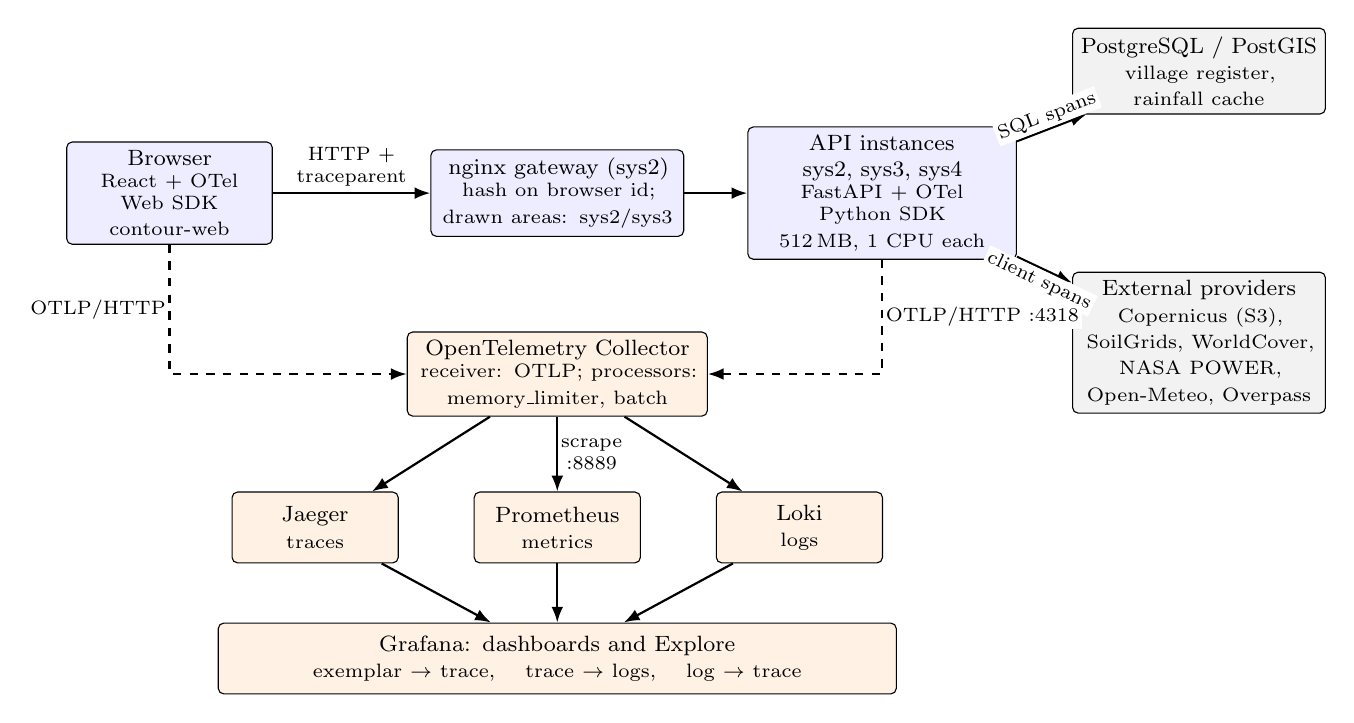
\begin{tikzpicture}[
      box/.style={draw, rounded corners=2pt, align=center, font=\footnotesize, minimum height=9mm, inner sep=3pt},
      app/.style={box, fill=blue!7},
      obs/.style={box, fill=orange!10},
      ext/.style={box, fill=gray!10},
      arr/.style={-{Latex[length=2mm]}, thick},
      lab/.style={font=\scriptsize, midway, fill=white, inner sep=1pt}]
    \node[app, text width=2.4cm] (web) {Browser\\\scriptsize React + OTel Web SDK\\\code{contour-web}};
    \node[app, text width=3.0cm, right=2.0cm of web] (gw) {nginx gateway (sys2)\\\scriptsize hash on browser id;\\drawn areas: sys2/sys3};
    \node[app, text width=3.2cm, right=0.8cm of gw] (api) {API instances sys2, sys3, sys4\\\scriptsize FastAPI + OTel Python SDK\\512\,MB, 1 CPU each};
    \node[ext, text width=3.0cm, above right=0.15cm and 0.7cm of api] (db) {PostgreSQL / PostGIS\\\scriptsize village register, rainfall cache};
    \node[ext, text width=3.0cm, below right=0.15cm and 0.7cm of api] (prov) {External providers\\\scriptsize Copernicus (S3), SoilGrids, WorldCover, NASA POWER, Open-Meteo, Overpass};
    \node[obs, text width=3.6cm, below=1.2cm of gw] (col) {OpenTelemetry Collector\\\scriptsize receiver: OTLP; processors:\\memory\_limiter, batch};
    \node[obs, text width=1.9cm, below left=0.95cm and 0.1cm of col] (jaeger) {Jaeger\\\scriptsize traces};
    \node[obs, text width=1.9cm, below=0.95cm of col] (prom) {Prometheus\\\scriptsize metrics};
    \node[obs, text width=1.9cm, below right=0.95cm and 0.1cm of col] (loki) {Loki\\\scriptsize logs};
    \node[obs, text width=8.4cm, below=0.75cm of prom] (graf) {Grafana: dashboards and Explore\\\scriptsize exemplar $\rightarrow$ trace, \quad trace $\rightarrow$ logs, \quad log $\rightarrow$ trace};
    \draw[arr] (web) -- node[lab, above=1pt, align=center] {HTTP +\\\code{traceparent}} (gw);
    \draw[arr] (gw) -- (api);
    \draw[arr] (api) -- node[lab, sloped, above] {SQL spans} (db);
    \draw[arr] (api) -- node[lab, sloped, below] {client spans} (prov);
    \draw[arr, dashed] (api) |- node[lab, pos=0.25, right] {OTLP/HTTP :4318} (col);
    \draw[arr, dashed] (web) |- node[lab, pos=0.25, left] {OTLP/HTTP} (col);
    \draw[arr] (col) -- (jaeger);
    \draw[arr] (col) -- node[lab, right, align=center] {scrape\\:8889} (prom);
    \draw[arr] (col) -- (loki);
    \draw[arr] (jaeger) -- (graf);
    \draw[arr] (prom) -- (graf);
    \draw[arr] (loki) -- (graf);
  \end{tikzpicture}
  \caption{Telemetry flow. Solid arrows are application traffic; dashed arrows are telemetry,
    exported over OTLP to one Collector, which routes each signal to its store.}
  \label{fig:arch}
\end{figure}

\subsection{Backend instrumentation}
All telemetry set-up lives in one module, \code{backend/app/core/telemetry.py}. It is
\emph{inert unless a collector is named}. Without \code{OTEL_EXPORTER_OTLP_ENDPOINT} (on the lab,
in the test suite, on a laptop) it installs nothing, and every helper is a no-op. With it, the
module creates the three SDK providers with batch exporters and installs the library
instrumentations. Everything else is configured through the standard OTel environment variables
(\code{OTEL_SERVICE_NAME}, \code{OTEL_RESOURCE_ATTRIBUTES}, \code{OTEL_METRIC_EXPORT_INTERVAL}),
so no Contour-specific settings were invented. Table~\ref{tab:instr} lists what is instrumented.

\begin{table}[!htb]
  \caption{What is instrumented, automatically and by hand}
  \label{tab:instr}
  \small
  \begin{tabular}{L{1.4cm}L{6.4cm}L{7.5cm}}
    \toprule
    Signal & Automatic (instrumentation libraries) & Manual (written for Contour) \\
    \midrule
    Traces & a server span per HTTP request (FastAPI), a span per background task, a client span
      per outgoing call (httpx: every data provider), a span per SQL statement (SQLAlchemy),
      context carried into thread pools (threading)
    & \code{analysis.job}, \code{analysis.queue_wait}, \code{analysis.area} /
      \code{analysis.contour}, one \code{stage.*} span per pipeline stage, \code{enrichment.*}
      per data layer, \code{rainfall.*} per rainfall source, \code{copernicus.tile} per terrain
      tile, \code{celery.worker_check}; the answer (tier, number of sites, expected water) as
      attributes \\
    Metrics & \code{http.client.request.duration} (httpx), \code{db.client.connections.usage}
      (SQLAlchemy)
    & request rate and latency to the last byte, stage, analysis and job-wait durations, jobs by
      final state, 503 refusals by reason, cache hits and misses, data tier, rainfall source
      outcomes, analysis slots in use, process memory \\
    Logs & every \code{logging} record, through OTel's logging handler
    & a structlog processor that sends each structured event to OTel with its trace and span id,
      after secrets are masked \\
    \bottomrule
  \end{tabular}
\end{table}

\paragraph{Spans that follow the pipeline.}
The pipeline already ran every stage through one helper (\code{_stage_runner} in
\code{contour_analysis.py}), so wrapping that helper in a span gave every stage a span and a
duration metric with one change. The four enrichment layers run in parallel threads under a 20\,s
deadline; their spans are children of \code{stage.enrichment} because the threading
instrumentation carries the trace context into the pool. Terrain tiles are read by GDAL, whose
HTTP client no Python instrumentation can see, so \code{copernicus.tile} spans were added by hand.
Without them a slow S3 read would appear only as unexplained time in the terrain stage.

\paragraph{Metrics.}
Table~\ref{tab:metrics} lists the custom metrics. Histograms use explicit bucket boundaries from
5\,ms to 60\,s, because the SDK's defaults stop at 10\,s and every cold analysis would land in
the last bucket. Attributes use low-cardinality values such as route \emph{templates} rather
than raw paths. Job ids and trace ids go on spans, never on metrics.

\begin{table}[!htb]
  \caption{Custom metrics (OTel name; Prometheus adds \codett{_seconds}, \codett{_total} and similar suffixes)}
  \label{tab:metrics}
  \small
  \begin{tabular}{L{5.3cm}L{1.7cm}L{3.1cm}L{4.8cm}}
    \toprule
    Metric & Type & Attributes & Answers \\
    \midrule
    \code{http.server.request.duration} & histogram & method, route, status & latency and request rate per endpoint \\
    \code{http.server.active_requests} & up-down counter & method & requests in flight \\
    \code{contour.stage.duration} & histogram & stage, outcome & which stage costs the most \\
    \code{contour.analysis.duration} & histogram & input, outcome & end-to-end analysis time \\
    \code{contour.job.queue_wait} & histogram & input & time spent waiting for a slot \\
    \code{contour.jobs} & counter & input, state & jobs done, partial or failed \\
    \code{contour.requests.rejected} & counter & reason & 503s: slot busy or queue full \\
    \code{contour.enrichment.layer.duration} & histogram & layer, outcome & slow or late data layers \\
    \code{contour.enrichment.tier} & counter & tier & how often an answer lacked a layer \\
    \code{contour.rainfall.source} & counter & source, outcome & which rainfall service answered \\
    \code{contour.cache.lookups} & counter & cache, result & cache hit ratio per cache \\
    \code{contour.analysis.slots} & gauge & state & analyses running, jobs waiting \\
    \code{process.memory.usage} & gauge & -- & resident memory against the 512\,MB limit \\
    \bottomrule
  \end{tabular}
\end{table}

\paragraph{Logs.}
Contour logs through structlog, which prints directly to stdout and bypasses Python's
\code{logging} module, so the standard OTel logging handler alone would have missed most log
lines. A small structlog processor sends a copy of every event to the OTel log pipeline, with the
event's fields as attributes. It sits after the redaction step, so a secret is masked in the
exported copy as well. The same processor adds \code{trace_id} and \code{span_id} to the console
line, so even \code{docker logs} output can be matched to a trace. Records from OTel's own
loggers are filtered out of the pipeline: exporting ``export failed'' through the exporter that
failed would loop for as long as the collector is down.

\paragraph{Errors carry their trace.}
Every response now carries an \code{X-Trace-Id} header, and every error body
(\code{application/problem+json}) quotes the same id, which the web page displays. A failed
background job records the exception on its span and reports its own trace id. A user who
reports ``trace ea5de5e4\ldots'' therefore gives the engineer the exact trace to open.

\subsection{Browser instrumentation}
The front end uses the OpenTelemetry Web SDK with the fetch instrumentation. Every API call
carries a \code{traceparent} header, so the server's spans continue the trace the browser
started, through the gateway, which forwards headers unchanged. One user action (\code{ui.run})
is one trace containing the job start, every status poll, the result and the follow-up map
layers. A browser has no asynchronous context propagation of its own, so the action's context is
re-entered around each \code{fetch} call, which is where the instrumentation reads it. The SDK
is a separate 21.8\,kB (gzipped) chunk, loaded only when the bundle is built with
\code{VITE_OTEL_TRACES_URL}. The lab's bundle does not contain it.

\subsection{Collector, backends and dashboard}
The Collector (\code{deploy/observability/otel-collector.yaml}) has one OTLP receiver, with CORS
enabled for the browser, and three pipelines. A \code{memory_limiter} processor stops it from
being OOM-killed under a burst, and \code{batch} groups data before export. Traces go to Jaeger
over OTLP. Metrics are exposed for Prometheus with resource attributes turned into labels, so any
metric can be split by instance, and in OpenMetrics format, so latency buckets carry
\emph{exemplars}: trace ids of sampled requests. Logs go to Loki's native OTLP endpoint. Grafana
is provisioned with the three data sources, cross-linked, and a 23-panel dashboard covering
traffic, the pipeline, capacity, logs and the telemetry pipeline itself.

\subsection{Deployment used for the demonstration}
The observability stack is a Docker Compose overlay on the project's four-system lab emulation
(\code{deploy/observability/compose.yml}), started with one command, \code{up.sh}. It mirrors
the lab deployment:
\begin{itemize}
  \item three API instances (sys2--sys4), each limited to 512\,MB and one CPU;
  \item the same nginx gateway, with drawn areas sent only to sys2 and sys3;
  \item PostgreSQL/PostGIS, as on sys4;
  \item the Collector, Jaeger, Prometheus, Loki and Grafana.
\end{itemize}
The backends were not deployed on the lab systems themselves. Each has 512\,MB of memory and a
1.5\,GB disk quota that the application already fills, and the lab offers no Docker. In
production the same three environment variables would point the instances at a collector on a
separate host; no code would change.

%% =====================================================================
\section{Tools, Libraries and Backend Services}
\label{sec:tools}
Table~\ref{tab:tools} lists everything used, with exact versions. All versions were at least two
weeks old when chosen. One exception was deliberate: Jaeger 2.21 removed the legacy query API
that Grafana's Jaeger data source still calls, so 2.20 is used.

\begin{table}[!htb]
  \caption{Tools, libraries and backends}
  \label{tab:tools}
  \small
  \begin{tabular}{L{5.6cm}L{1.5cm}L{8.2cm}}
    \toprule
    Component & Version & Role \\
    \midrule
    \code{opentelemetry-api}, \code{-sdk} & 1.44.0 & Python API and SDK: providers, batch processors, metric reader \\
    \code{opentelemetry-exporter-otlp-proto-http} & 1.44.0 & OTLP over HTTP/protobuf (gRPC avoided: 30\,MB of native code on a 512\,MB system) \\
    \code{opentelemetry-instrumentation-*} & 0.65b0 & FastAPI, httpx, SQLAlchemy, threading, logging handler \\
    \code{@opentelemetry/sdk-trace-web} & 2.11.0 & browser tracer provider \\
    \code{@opentelemetry/instrumentation-fetch} & 0.222.0 & browser spans and \code{traceparent} on every API call \\
    \code{@opentelemetry/exporter-trace-otlp-http} & 0.222.0 & browser span export \\
    OpenTelemetry Collector (contrib) & 0.160.0 & receives OTLP; routes each signal to its store \\
    Jaeger & 2.20.0 & trace storage and the trace UI \\
    Prometheus & 3.13.3 & metric storage and query (PromQL), exemplar storage \\
    Loki & 3.6.15 & log storage, native OTLP ingestion with structured metadata \\
    Grafana & 12.4.12 & dashboards and cross-signal exploration \\
    PostgreSQL / PostGIS & 16 / 3.4 & the application's database (traced as SQL spans) \\
    nginx & 1.27.5 & the gateway; forwards \code{traceparent} \\
    \bottomrule
  \end{tabular}
\end{table}

%% =====================================================================
\section{Running and Verifying the Implementation}
\label{sec:verify}

\paragraph{Running.}
\code{deploy/observability/up.sh} starts the emulation with telemetry. The script
\code{scripts/telemetry_demo.py} then plays the part of several users:
\begin{itemize}
  \item a warm analysis of the sample area, and a cold analysis of a randomly placed area that
    no instance has seen;
  \item the sample contour survey uploaded as a job;
  \item four errors: an unknown job (404), a rectangle over the sea (422), one over 100\,km$^2$
    (413) and a file that is not KML;
  \item an overload burst on one instance: a slow analysis holding its only slot, two synchronous
    calls refused with 503, and two jobs queued behind it;
  \item optionally (\code{--soak}), steady traffic from nine simulated browsers for several minutes.
\end{itemize}
During one soak, the API on sys3 was stopped for 53\,s to test failover. All 340 analyses in
that soak completed.

\paragraph{Verifying.}
The same script then reads every signal back from the backend that stores it. All 11 checks
passed (Table~\ref{tab:checks}).

\begin{table}[!htb]
  \caption{Verification against the backends (\codett{telemetry_demo.py}, after 5 minutes of traffic)}
  \label{tab:checks}
  \small
  \begin{tabular}{L{6.9cm}L{1.2cm}L{7.2cm}}
    \toprule
    Check & Result & Evidence \\
    \midrule
    Jaeger: the API is a traced service & PASS & services \code{contour-api}, \code{contour-web} \\
    Jaeger: pipeline spans recorded & PASS & 39 operations, none missing \\
    Jaeger: a job's trace holds the 202 and every stage & PASS & 50 of 50 job traces \\
    Jaeger: spans say which instance served & PASS & sys2, sys3 \\
    Prometheus: stage durations recorded & PASS & 1\,576 stage samples \\
    Prometheus: request metrics recorded & PASS & 2\,213 requests \\
    Prometheus: memory per instance & PASS & sys2 358\,MB, sys3 324\,MB, sys4 370\,MB \\
    Prometheus: 503 refusals counted & PASS & 2 refused \\
    Prometheus: provider calls measured & PASS & 7 hosts, including 4 Overpass mirrors \\
    Loki: logs arrived with trace ids & PASS & 200 lines checked \\
    Loki $\leftrightarrow$ Jaeger: a log line opens its trace & PASS & 34 job traces have log lines \\
    \bottomrule
  \end{tabular}
\end{table}

\paragraph{Automated tests.}
39 new tests run the real application with in-memory exporters and assert the properties this
report relies on:
\begin{itemize}
  \item telemetry is inert without a collector;
  \item a job's trace descends from the request that started it and contains every stage;
  \item a job-start request span ends before its background job does, and its latency metric
    excludes the job;
  \item an error body's trace id is the trace's id;
  \item log records carry the trace id, and secrets are masked before export;
  \item the environment's resource attributes override the defaults.
\end{itemize}
The full backend suite (1\,531 tests) passes with the instrumentation in place, as do lint,
formatting and type checks.

%% =====================================================================
\section{Screenshots and What They Show}
\label{sec:shots}
All screenshots are from this project running as described above, captured with headless Chrome
on 16 October 2026. Trace ids in the captions can be looked up in Jaeger while the stack is
running.

\subsection{One user action, end to end}
Figure~\ref{fig:ui} is the workspace after a user drew a 1.65\,km$^2$ rectangle that its
instance had never analysed, and pressed \emph{Run}. Figure~\ref{fig:e2e} is the trace of that
action.

\noindent\textbf{What Figure~\ref{fig:e2e} shows.} One trace joins the browser
(\code{contour-web}, orange) and the API (\code{contour-api}, blue) because the browser's
\code{traceparent} header reached the API through the gateway. The job's spans hang under the
202 request. The nesting reads like the pipeline itself, and the bar lengths show where the
27\,seconds went:
\begin{itemize}
  \item 20\,s of enrichment, bounded by the deadline;
  \item 6\,s of terrain download, cold because each instance keeps its own cache;
  \item well under a second for the actual hydrology.
\end{itemize}
The rainfall layer took only 54\,ms because its cache is the shared database: another instance
had already fetched that grid cell.

\begin{figure}[H]
  \centering
  \includegraphics[width=\linewidth]{figures/ui-run.png}
  \caption{The application: a freshly drawn rectangle, analysed. Site \#1, its 5.3\,ha catchment
    and its expected 2\,251\,m$^3$ a year are drawn on the map.}
  \label{fig:ui}
\end{figure}

\begin{figure}[H]
  \centering
  \includegraphics[width=0.92\linewidth]{figures/trace-e2e.png}
  \caption{Jaeger: the trace of that \emph{Run} (\codett{25fe2614...}), with 83 spans from two
    services. The browser's \codett{ui.run} span (27.2\,s) contains its \codett{POST}, which the API
    on sys3 answered with 202 in 3.3\,ms. The background job follows: the terrain stage (the
    Copernicus tile read from S3, 6.0\,s) and the enrichment stage, stopped at its 20.0\,s
    deadline, with the soil (3.2\,s), land-cover (4.6\,s) and rainfall (54\,ms, two cache hits
    in PostgreSQL) layers inside. The OpenStreetMap layer's Overpass calls ran past the deadline.
    Below the job, each browser status poll pairs with the server span it caused.}
  \label{fig:e2e}
\end{figure}

\begin{figure}[H]
  \centering
  \includegraphics[width=\linewidth]{figures/trace-overpass.png}
  \caption{A client span from the httpx instrumentation, expanded: the OpenStreetMap request,
    \codett{POST https://overpass-api.de/api/interpreter}, took 40.4\,s for HTTP 200. Its parent,
    \codett{enrichment.existing_water}, lasted 1.2\,minutes, long after the analysis had finished
    without it.}
  \label{fig:overpass}
\end{figure}

\noindent\textbf{What Figure~\ref{fig:overpass} shows.} Automatic instrumentation records the
method, URL, status and timing of every outgoing call. Here it names the slow dependency: the
Overpass service took twice the whole enrichment budget. The design (a deadline, then continue
without the layer) protected the user from it, and the trace makes that visible.

\begin{figure}[H]
  \centering
  \includegraphics[width=\linewidth]{figures/trace-sql.png}
  \caption{A SQL span from the SQLAlchemy instrumentation: the rainfall-cache lookup, with the
    statement, database, server and the process that ran it (\codett{service.instance.id=sys3}).}
  \label{fig:sql}
\end{figure}

\noindent\textbf{What Figure~\ref{fig:sql} shows.} Database work appears in traces without any
hand-written code. The statement shown is the cached-rainfall query keyed by provider grid cell,
taking 28\,ms. The \emph{Process} line shows the resource attributes that identify the instance.

\subsection{Finding traces}
\begin{figure}[H]
  \centering
  \includegraphics[width=\linewidth]{figures/jaeger-search.png}
  \caption{Jaeger search for the browser's \codett{ui.run} traces. Each spans two services; the
    second has 4 error spans (the rejected upload of Section~\ref{sec:errors}); the scatter plot
    places them by duration.}
  \label{fig:search}
\end{figure}

\noindent\textbf{What Figure~\ref{fig:search} shows.} Traces are searchable by service,
operation, duration and attributes. Because the answer is recorded on the analysis span, one can
search for example for \code{contour.tier=terrain_only} to list every analysis that lacked a data
layer, or for \code{contour.problem.status=503}.

\subsection{Metrics: the Grafana dashboard}
Figures~\ref{fig:dash-traffic}--\ref{fig:dash-capacity} show the dashboard after 30 minutes of
scripted traffic, soak traffic and the failover test.

\begin{figure}[H]
  \centering
  \includegraphics[width=\linewidth]{figures/dash-traffic.png}
  \caption{Traffic: request rate, p95 latency (13.7\,ms), 5xx ratio (0.2\,\%: the deliberate
    503s), 470 jobs finished; requests by route, latency by route with exemplar dots, responses
    by status code, and requests by instance.}
  \label{fig:dash-traffic}
\end{figure}

\noindent\textbf{What Figure~\ref{fig:dash-traffic} shows.} These are the RED metrics (rate,
errors, duration) of the API. The status-code panel includes the 4xx and 503 responses the
scripts provoked. The per-instance panel (bottom right) records the failover. At about 16:07 the
API on sys3 (yellow) was stopped; its browsers, hashed to it by the gateway, moved to sys2
(green) within seconds, and sys3's traffic returned when it restarted 53\,s later. The dots on the
latency panel are exemplars: clicking one opens the trace of that exact request.

\begin{figure}[H]
  \centering
  \includegraphics[width=\linewidth]{figures/dash-pipeline.png}
  \caption{Pipeline: mean duration per stage and per enrichment layer, analysis duration by input
    type, cache hit ratios, outgoing provider calls by host and status, and the data tier of
    finished analyses.}
  \label{fig:dash-pipeline}
\end{figure}

\noindent\textbf{What Figure~\ref{fig:dash-pipeline} shows.} Interpolating a contour survey
(1.54\,s) and enrichment dominate. The \code{existing_water (late)} bar (56\,s) is the
OpenStreetMap layer arriving after its deadline. Caches answer 99\,\% of lookups, which is why a
warm analysis takes a second instead of thirty. The provider panel shows Overpass mirrors failing
(502, 500, 504) before one answers: the provider's fallback, measured.

\begin{figure}[H]
  \centering
  \includegraphics[width=\linewidth]{figures/dash-capacity.png}
  \caption{Capacity: resident memory per instance against the 512\,MB limit, analyses running and
    jobs waiting, 503 refusals per minute by reason, and job wait time.}
  \label{fig:dash-capacity}
\end{figure}

\noindent\textbf{What Figure~\ref{fig:dash-capacity} shows.} These panels check the lab's
memory budget directly. Each instance stayed between 250 and 470\,MB, below the red 512\,MB line.
Each instance runs at most one analysis; during the overload burst the second panel shows jobs
waiting, the third shows the two refused calls (\code{slots_busy}), and the fourth shows the
queued jobs' 30--45\,s wait.

\begin{figure}[H]
  \centering
  \includegraphics[width=\linewidth]{figures/prometheus-table.png}
  \caption{Prometheus, queried directly: calls to external providers per instance, host and
    status code since each instance started.}
  \label{fig:prom}
\end{figure}

\noindent\textbf{What Figure~\ref{fig:prom} shows.} This is the raw data behind the dashboard.
Prometheus stores each combination of attributes as a time series. On sys3, the OpenStreetMap
request was refused by four Overpass mirrors (\code{overpass-api.de} 502,
\code{overpass.kumi.systems} 500, \code{overpass.private.coffee} 500, \code{maps.mail.ru} 504)
before \code{maps.mail.ru} answered.

\subsection{Logs and their correlation with traces}
\begin{figure}[H]
  \centering
  \includegraphics[width=\linewidth]{figures/loki-trace.png}
  \caption{Grafana Explore on Loki: every log line of one trace (\codett{25fe2614...}, the
    \emph{Run} of Figure~\ref{fig:e2e}), from \codett{area analysis job accepted} to
    \codett{overpass answered}. The expanded line shows its fields and a \emph{View trace} link to
    Jaeger.}
  \label{fig:loki}
\end{figure}

\noindent\textbf{What Figure~\ref{fig:loki} shows.} The log query is a trace id. Loki returns the
nine lines written while that action was handled, from different modules, on sys3. The
structured fields (\code{job_id}, \code{bbox}, \code{logger_name}) are searchable, and the
derived \emph{View trace} link goes from a log line to its trace.

\begin{figure}[H]
  \centering
  \includegraphics[width=\linewidth]{figures/dash-logs.png}
  \caption{The dashboard's log panels: recent warnings and errors across all instances, and log
    volume by severity.}
  \label{fig:dash-logs}
\end{figure}

\noindent\textbf{What Figure~\ref{fig:dash-logs} shows.} Warnings from all three instances
appear in one place: Overpass mirrors failing, the provoked \code{request_failed} problems, and
the rejected KML file.

\begin{figure}[H]
  \centering
  \includegraphics[width=\linewidth]{figures/terminal.png}
  \caption{Raw output on the command line. (a) The Collector's debug exporter, one line per batch
    received: 24 spans from 3 instances, 8 log records, 103 metric points. (b) An API instance's
    console log: each line carries its \codett{trace_id} and \codett{span_id}.}
  \label{fig:terminal}
\end{figure}

\noindent\textbf{What Figure~\ref{fig:terminal} shows.} This is the lowest-level evidence that
data flows. Part (a) shows the Collector receiving all three signals from all three instances
every few seconds. Part (b) shows that the trace id appears even in plain container logs, so a
line from \code{docker logs} can be taken to Jaeger.

\begin{figure}[H]
  \centering
  \includegraphics[width=\linewidth]{figures/dash-traces.png}
  \caption{Recent analysis jobs, listed from Jaeger in Grafana, and the Collector's own metrics:
    spans, metric points and log records received per second, and anything refused.}
  \label{fig:dash-traces}
\end{figure}

\noindent\textbf{What Figure~\ref{fig:dash-traces} shows.} The telemetry pipeline monitors
itself. A drop in received spans, or a non-zero ``refused'' line, would mean that telemetry
itself is failing, which matters because an empty dashboard can look the same as a healthy,
idle system.

\subsection{Errors, from the screen to the line of code}
\label{sec:errors}
\begin{figure}[H]
  \centering
  \includegraphics[width=\linewidth]{figures/ui-rejected.png}
  \caption{A rejected upload: the page shows the API's reason and \codett{trace ea5de5e4...}.}
  \label{fig:ui-rejected}
\end{figure}

\begin{figure}[H]
  \centering
  \includegraphics[width=0.84\linewidth]{figures/trace-rejected.png}
  \caption{The same id in Jaeger. The browser's \codett{ui.run} and the server's
    \codett{stage.parse} are marked as errors; the expanded span holds the exception event with its
    message and full stack trace, down to \codett{contour_kml.py}, line 403.}
  \label{fig:trace-rejected}
\end{figure}

\noindent\textbf{What Figures~\ref{fig:ui-rejected} and~\ref{fig:trace-rejected} show.} This is
the debugging workflow the instrumentation makes possible:
\begin{enumerate}
  \item The user sees an error and a trace id.
  \item That id opens one trace containing the browser action, the 202, the background job and
    the failing stage.
  \item The failing span holds the stack trace, which the user was deliberately never shown.
\end{enumerate}
The trace also shows something the error message does not: the upload's 202 itself took 6.3\,s
(Section~\ref{sec:found}).

\begin{figure}[H]
  \centering
  \includegraphics[width=0.94\linewidth]{figures/trace-sea.png}
  \caption{A rectangle drawn over the Bay of Bengal (422): the four \codett{copernicus.tile} spans
    each failed with \codett{RasterioIOError}, because the buffered area crosses four 1-degree
    tiles, none of which exists over the sea.}
  \label{fig:sea}
\end{figure}

\noindent\textbf{What Figure~\ref{fig:sea} shows.} An input error that is not a server fault.
The 422 and the span attributes explain it: no land, so no terrain tiles.

\subsection{Overload}
\begin{figure}[H]
  \centering
  \includegraphics[width=0.88\linewidth]{figures/trace-queued.png}
  \caption{A job started while its instance's only analysis slot was taken: the 202 took 2.7\,ms,
    \codett{analysis.queue_wait} lasted 30\,s, and the analysis itself 232\,ms.}
  \label{fig:queued}
\end{figure}

\noindent\textbf{What Figure~\ref{fig:queued} shows.} The overload policy at work. Jobs queue
instead of crashing a 512\,MB instance, and the trace separates the time spent waiting from the
time spent working. Without the \code{queue_wait} span, this would look like a 30\,s analysis.

%% =====================================================================
\section{What the Data Revealed}
\label{sec:findings}

\subsection{Problems found by the telemetry, and fixed}
\label{sec:found}
\paragraph{1. Request spans included background jobs.}
A job start returns 202 in a few milliseconds, but its server span lasted as long as the whole
analysis, about 20\,s. Starlette runs a route's background task inside the same ASGI call, and
the OTel ASGI middleware ends its span, and records its latency histogram, when that call
returns. The fix is a small middleware that ends the request span and records latency when the
last byte of the response is sent. The job then appears as a child span that outlives its
request (Figure~\ref{fig:queued}), and the latency metric shows what the client actually waited.
A test checks this.

\paragraph{2. Contour uploads took 6.1\,s to start.}
Comparing job-start latencies in Jaeger showed that drawn-area starts took a median of 2.7\,ms
(40 traces) but contour-upload starts took 6.0--6.3\,s, with no child span to explain the
difference. Adding a span around the one step only uploads perform, a check for a Celery worker,
located it. Figure~\ref{fig:upload}a shows 6.0\,s of the 6.1\,s inside \code{celery.worker_check}:
the emulation pointed the broker at a dead port, assuming it would fail instantly, but Celery
retries. Configured as on the lab, with no broker, the upload starts in 84\,ms
(Figure~\ref{fig:upload}b), most of it receiving the 6.7\,MB file.

\begin{figure}[H]
  \centering
  \begin{subfigure}{\linewidth}
    \includegraphics[width=\linewidth]{figures/trace-upload-before.png}
    \caption{Before: 6.1\,s to answer 202, of which 6.0\,s in \codett{celery.worker_check}.}
  \end{subfigure}
  \par\medskip
  \begin{subfigure}{\linewidth}
    \includegraphics[width=\linewidth]{figures/trace-upload-after.png}
    \caption{After: 84\,ms; the job starts at once.}
  \end{subfigure}
  \caption{Contour upload starts, before and after the fix the trace pointed to.}
  \label{fig:upload}
\end{figure}

\paragraph{3. The gateway sent drawn areas to the wrong instance.}
Drawn areas must go only to sys2 and sys3, which on the lab hold the terrain tiles. After the
failover test restarted sys3's container, a trace showed a drawn-area request served by
\code{service.instance.id=sys4} (Figure~\ref{fig:misrouted}). nginx resolves upstream host
names once, at start-up. The restarted container came back with a new address, and its old
address had passed to sys4's container, so nginx kept sending ``sys3'' traffic to sys4.
Functional checks could not catch this, because sys4 answers correctly in the emulation; only
the instance attribute on the span exposed it. The demo's gateway is now generated with
\code{--docker-dns}, which makes nginx keep re-resolving the container names (\code{resolve},
nginx $\geq$ 1.27.3). After further restarts, drawn areas stayed on sys2 and sys3. The same
mechanism broke the lab gateway on 27 September, when a restart reshuffled internal addresses;
the lab gateway now uses published ports, which a restart does not change.

\begin{figure}[H]
  \centering
  \includegraphics[width=\linewidth]{figures/trace-misrouted.png}
  \caption{The trace that exposed the misrouting: \codett{POST /api/v1/analysis/area} served at
    \codett{172.18.0.10}, which belonged to \codett{service.instance.id=sys4}, an instance outside
    the drawn-area pool.}
  \label{fig:misrouted}
\end{figure}

\paragraph{4. A slow external dependency.}
The OpenStreetMap Overpass service took 22--40\,s per request and was often refused by mirrors
(Figures~\ref{fig:overpass} and~\ref{fig:prom}). This is outside the project's control. The
telemetry shows that the 20\,s enrichment deadline contained it, at the cost of the
building-and-road exclusions for that run, and makes the service's behaviour measurable over time.

\subsection{How the system behaves}
\begin{itemize}
  \item \textbf{Where time goes.} A warm drawn area is analysed in about a second. A cold one
    takes 26--34\,s, of which 20\,s is the enrichment deadline, about 6\,s is the terrain
    download, and less than a second is the hydrology.
  \item \textbf{Caches.} Terrain, soil, land cover and OpenStreetMap caches are per instance, so
    the same area is cold on a second instance. Rainfall is cached in the shared database, so it
    is warm everywhere.
  \item \textbf{Capacity.} Memory stayed below 470\,MB of 512\,MB on every instance. Overload
    produced 503s and queueing, never a crash.
  \item \textbf{Failover.} 340 of 340 analyses completed while one instance was stopped for 53\,s.
\end{itemize}

\subsection{What instrumentation costs}
To measure the overhead, sys4 was recreated alternately with telemetry on and with
\code{OTEL_SDK_DISABLED=true}, and the same benchmark was run each time: 25 warm analyses and
300 light requests, two runs per mode (Table~\ref{tab:overhead}).

\begin{table}[!htb]
  \caption{Overhead on one instance (512\,MB, 1 CPU); ranges over two runs per mode}
  \label{tab:overhead}
  \small
  \begin{tabular}{L{5.6cm}L{2.7cm}L{2.7cm}L{3.9cm}}
    \toprule
    Measure & Telemetry off & Telemetry on & Cost \\
    \midrule
    Resident memory, idle & 255--256\,MB & 264\,MB & +8--9\,MB \\
    Resident memory, peak after the benchmark & 298\,MB & 307--308\,MB & +10\,MB (2\,\% of 512\,MB) \\
    Warm analysis, median & 0.277--0.280\,s & 0.285--0.288\,s & +8\,ms ($\approx$3\,\%) \\
    Light request (\code{GET /health/features}), median & 0.31--0.42\,ms & 0.51--0.52\,ms & +0.1--0.2\,ms \\
    \bottomrule
  \end{tabular}
\end{table}

The cost is small against the lab's budget. Export runs on background threads, so a slow or
unavailable collector costs requests nothing. If the cost of traces ever mattered, head sampling
(\code{OTEL_TRACES_SAMPLER=parentbased_traceidratio}) would reduce it without code changes.

\subsection{How OpenTelemetry helps monitor, debug and analyse the application}
\begin{itemize}
  \item \textbf{Monitoring.} Request rate, errors, latency, queue depth, 503 refusals and memory
    are continuous metrics that alerts can watch, for example ``memory above 450\,MB'' or ``any
    \code{queue_full} refusal''. They summarise thousands of requests cheaply.
  \item \textbf{Debugging.} A trace answers what a log line cannot: which instance, which stage,
    which external call, and in what order, across processes. The trace id ties together what
    the user saw, the spans and the log lines. Two of the defects above produced no error at
    all; they were found only because the trace showed time or routing that did not fit.
  \item \textbf{Analysis.} The same data answers design questions: whether to share caches
    between instances, whether the 20\,s deadline is right, and how close to the memory limit
    the system runs.
  \item \textbf{Independence from vendors.} The application speaks only OTLP. Replacing Jaeger
    with another trace store, or sending a copy to a cloud service, is a Collector configuration
    change.
\end{itemize}

\subsection{Limitations}
\begin{itemize}
  \item The nginx hop forwards the trace context but emits no spans of its own (the nginx OTel
    module would add them).
  \item Celery workers and GDAL's internals are covered only by manual spans.
  \item Jaeger keeps traces in memory, which is enough for a demonstration but not for production.
  \item The browser exports directly to the Collector; in production it would go through the
    gateway.
  \item Every trace is recorded (sampling at 100\,\%).
  \item The lab deployment itself does not export telemetry, because its memory and disk quota
    leave no room for the backends. It would need a collector on another host.
\end{itemize}

%% =====================================================================
\section{Conclusion}
Contour now produces traces, metrics and logs through OpenTelemetry, from the browser to the
database and the external data services. The data is collected by one Collector, stored in
Jaeger, Prometheus and Loki, and explored in Grafana, where the three signals link to each other.
The implementation is inert by default, is configured only through the standard OTel variables,
costs about 10\,MB and 3\,\% of an analysis, and is covered by tests and an end-to-end
verification script. Its most convincing result is what it found: a request metric that
misreported job starts, a 6\,s delay on every contour upload, a gateway sending work to the
wrong instance, and a slow external service. None of these was visible in logs or functional
tests, and each was clear in a single trace.

%% =====================================================================
\section{AI Tool Usage Declaration}
% CHECK: this declaration is yours to make; edit it to match exactly how you used AI tools.
Claude (Anthropic), used through the Claude Code assistant, helped with this assignment: choosing
the libraries and backends, writing the instrumentation, tests, Collector and Grafana
configuration and demonstration scripts, running and debugging the stack, capturing the
screenshots, and drafting this report. The design decisions, the review of every result and the
final text are my own responsibility, and I can explain each part of the implementation.

%% =====================================================================
\begin{thebibliography}{9}
\bibitem{otel} OpenTelemetry Authors. \emph{OpenTelemetry Specification} and documentation.
  \url{https://opentelemetry.io/docs/}
\bibitem{semconv} OpenTelemetry Authors. \emph{Semantic Conventions for HTTP spans and metrics}.
  \url{https://opentelemetry.io/docs/specs/semconv/http/}
\bibitem{w3c} W3C. \emph{Trace Context}, W3C Recommendation, 2021.
  \url{https://www.w3.org/TR/trace-context/}
\bibitem{dapper} B.~H. Sigelman et al. \emph{Dapper, a Large-Scale Distributed Systems Tracing
  Infrastructure}. Google Technical Report, 2010.
\bibitem{jaeger} Jaeger Authors. \emph{Jaeger documentation}. \url{https://www.jaegertracing.io/docs/}
\bibitem{prom} Prometheus Authors. \emph{Prometheus documentation}. \url{https://prometheus.io/docs/}
\bibitem{loki} Grafana Labs. \emph{Loki: ingesting logs with OpenTelemetry}.
  \url{https://grafana.com/docs/loki/latest/send-data/otel/}
\end{thebibliography}

\end{document}
